\documentclass[twocolumn,10pt]{article}
\usepackage[T1]{fontenc}
\usepackage[utf8]{inputenc}
%\usepackage[english]{babel}
\usepackage{biblatex}
\usepackage[margin=1in]{geometry}
\setlength{\columnsep}{33pt}
\setcounter{secnumdepth}{1}
\usepackage{minipage-marginpar}
\newcommand\vfilbreak[1]{\vskip 0pt plus #1 \penalty-200 \vskip 0pt plus -#1}
\newenvironment{mpmp}[1]
               {\begin{minipagewithmarginpars}{#1}}
               {\end{minipagewithmarginpars}}
\usepackage{morefloats}
\usepackage{booktabs}
\usepackage{color}
\usepackage{graphicx}

\title{Lung Cancer detection with U-Net/Faster R-CNN \\
nodule/region of interest proposal}
\author{Jay Destories, Jason Fan, Alex Tong}
\date{March 2017}

\newcommand{\red}[1]{{\color{red}#1}}
\newcommand{\temp}[1]{{\red{#1}\\}}

\begin{document}

\maketitle
\section{Introduction and \\Problem~Statement}
The problem with segmentation and structure identification within the field of 
biomedical imaging has become a well developed and very active field in the past
years. In 2016 and 2015, the LUng Nodule Annotation (LUNA) challenge and 
SPIE Lungx challenge, asked researchers to develop models to identify pulmonary 
nodules in lung CT slices. In the 2016 LUNA Challenge, researchers gained access
to annotated CT slices that identified abnormal nodules but did not release data
about the malignancy of the nodles. In the 2015 SPIE less than 80 CT annotated 
images of malignant nodules were released to the public.

However, with the 2017 Kaggle Data Science Bowl, a large\red{ish} dataset of
1000+ lung CT images in DICOM format was finally released with cancer/no cancer 
labels. Preliminary investigations by Kaggle members
using 3D-convolutional neural nets have already begun. There is one caveat to this 
dataset; location of malignant nodules are not labeled. 

Inspired by recent work in biomedical image segmentation, region proposal 
networks and multiple instance learning for whole mammogram classification,
We seek to present a novel pipeline for cancer detection by combining
region proposal and multiple instance learning (MIL).

\section{Method/Algorithm/Pipeline}

\temp{TODO: fix the diagram - its 6x6x256, and also add FCNN to list of ROI nets}
% \temp{PIPELINE: NODULE EXTRACTION -> CNN -> CANCER CLASSIFICATION}
% \temp{Will we even use RNN? If so is UNET an RNN?}
% \temp{What kind of augmentations can we do in 3d? in the z axis?}

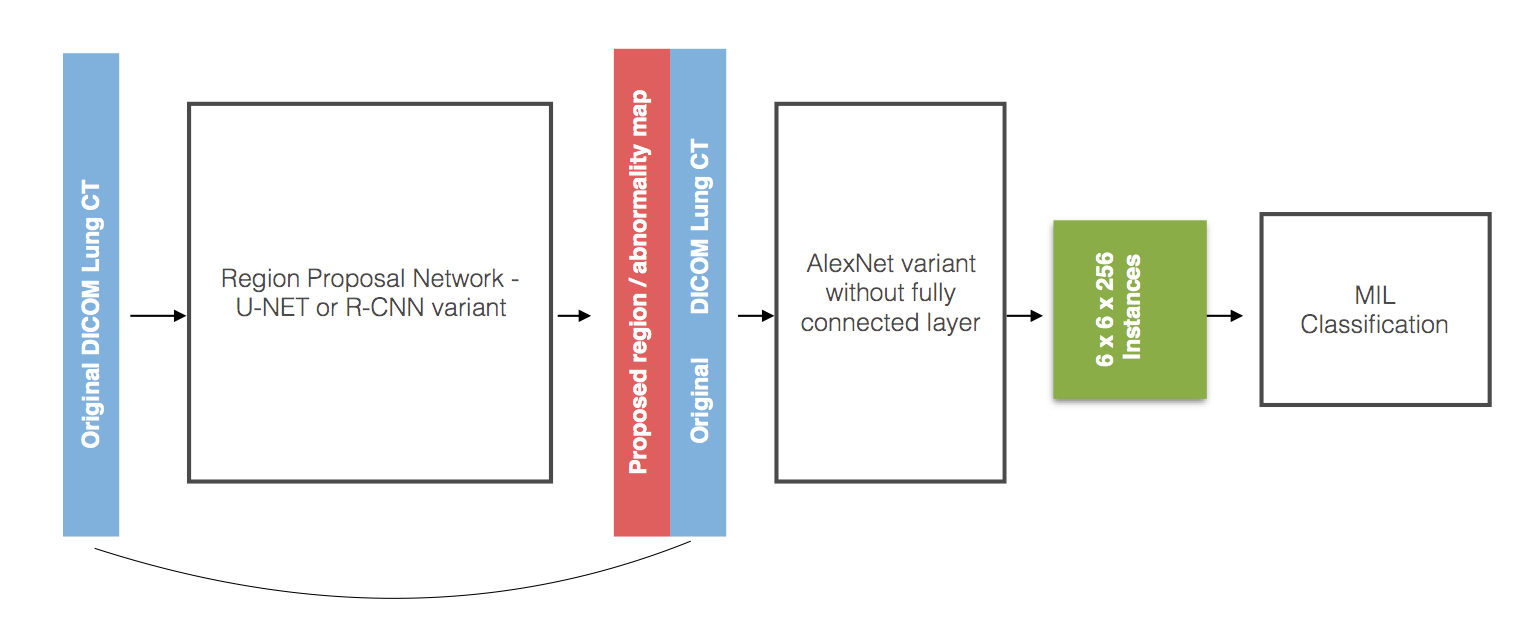
\includegraphics[width=\columnwidth]{img/architecture.png}

We will enhance multiple instance learning (MIL) by combining
MIL with region proposal. We plan to leverage state of the 
art region proposal networks to propose regions and implicitly weight instances 
consumed by a downstream MIL classifier.

In our pipeline a region proposal network trained on the LUNA dataset propose
abnormal regions in CT slices. These regions are composed with 
DICOM images are then fed into an MIL classifier that leverages AlexNet and 
is based on the work on mammogram classification by Zhu et. al.

\subsection{Region Proposal Networks}
We have three region proposal/image segmentation techniques we want to investigate.
We will tune one segmentation/region proposal network for our final pipeline. 

The first pipeline we will test is U-Net, a CNN for biomedical
segmentation developed by Brox et. al \red{add ref}. The second pipeline we will test
is the fully convolutional neural network developed by Darrell et al \red{add ref}.
(Jay and Jason will be investigating this network as a paper presentation). And
the third pipeline we will test is Faster R-CNN developed by He et. al \red{add ref}.

\subsection{Multiple Instance Learning}
We will adapt MIL techniques developed for mammogram classification developed by
Lou et. al \red{add ref}. Their implementation feeds the 6 by 6 by 256 output of the last
convolutional layer of AlexNet as instances that are then 

\section{Datasets}
The number of lung CT scans available to us is very low. The total number of examples
available are many orders of magnitudes smaller than the size of datasets for modern,
state of the art classification challenges such as ImageNet or MSCOCO. 

Listed below are the datsets we will leverage to train our classification/nodule
extraction model.

\begin{center}
\begin{tabular}{lll}
  \toprule
  Dataset & \# CT scans & Label Type\\
  \midrule
  Kaggle&1000+&Cancer/No-cancer\\
  LIDC-IDRI&888?&Nodule annotation\\
  NLST&?&?\\
  SPIE&80&Nodule annotation\\
\end{tabular}
\end{center}

\subsection{Kaggle Data Science Bowl - (Kaggle)}
\subsection{Lung Image Database Consortium image collection - (LIDC-IDRI)}
\subsection{National Lung Screening Trial - (NLST)}
\subsection{SPIE Lungx Challenge - (SPIE)}

\section{Goals and Evaluation}

The main challenge that we face in lung cancer detection 

\temp{Goals:?}
\temp{Tuning Faster/fast RNN or YOLO to detect nodules}
\temp{Using Alex-net or other 2GPU methods to train cancer classifier}
\temp{Find ways to reduce false positive/false negatives}

\temp{Visualizations of 3D convolutions?}
\temp{Comparison between plain CNN vs. nodule extraction -> CNN? }
\temp{Comparison between U-NET vs tuned FASTER R-CNN?}
\temp{}
\temp{
	1) Nodule extraction with u-net, r-cnn roi proposal, or another pre-trained
	model. TODO: what will be the extracted features be?! \\
	2) leverage 2 GPU with alex-net like architecture to classify cancer
	instances, we really dont have more data so we might have to train on the
	kaggle dataset.
}
\temp{Evaluate and visualize how region proposal/abnormality proposal actually
affects MIL classifiers}
\temp{Evaluate how our technique circumnavigates the problem of having sparse,
non-homogeneous data}

\section{About us}
\temp{buncha kiddos who have no idea about anything}

\section{Related Work}

\section{Questions and challenges}
\begin{enumerate}
	\item What will the output of node-extraction be like?
	\item What kind of novelty will we bring to the table?
	\item How will we deal with the small dataset(s)?
\end{enumerate}
\end{document}